\documentclass [12pt, a4paper] {article}
\usepackage[utf8x]{inputenc}
\usepackage[english,russian]{babel}
\usepackage[T2A]{fontenc}
\usepackage {graphicx}

%\let\stdsection\section
%\renewcommand\section{\newpage\stdsection}
\begin {document}

\thispagestyle {empty}

\begin {center}
    \ \vspace{-4cm}

    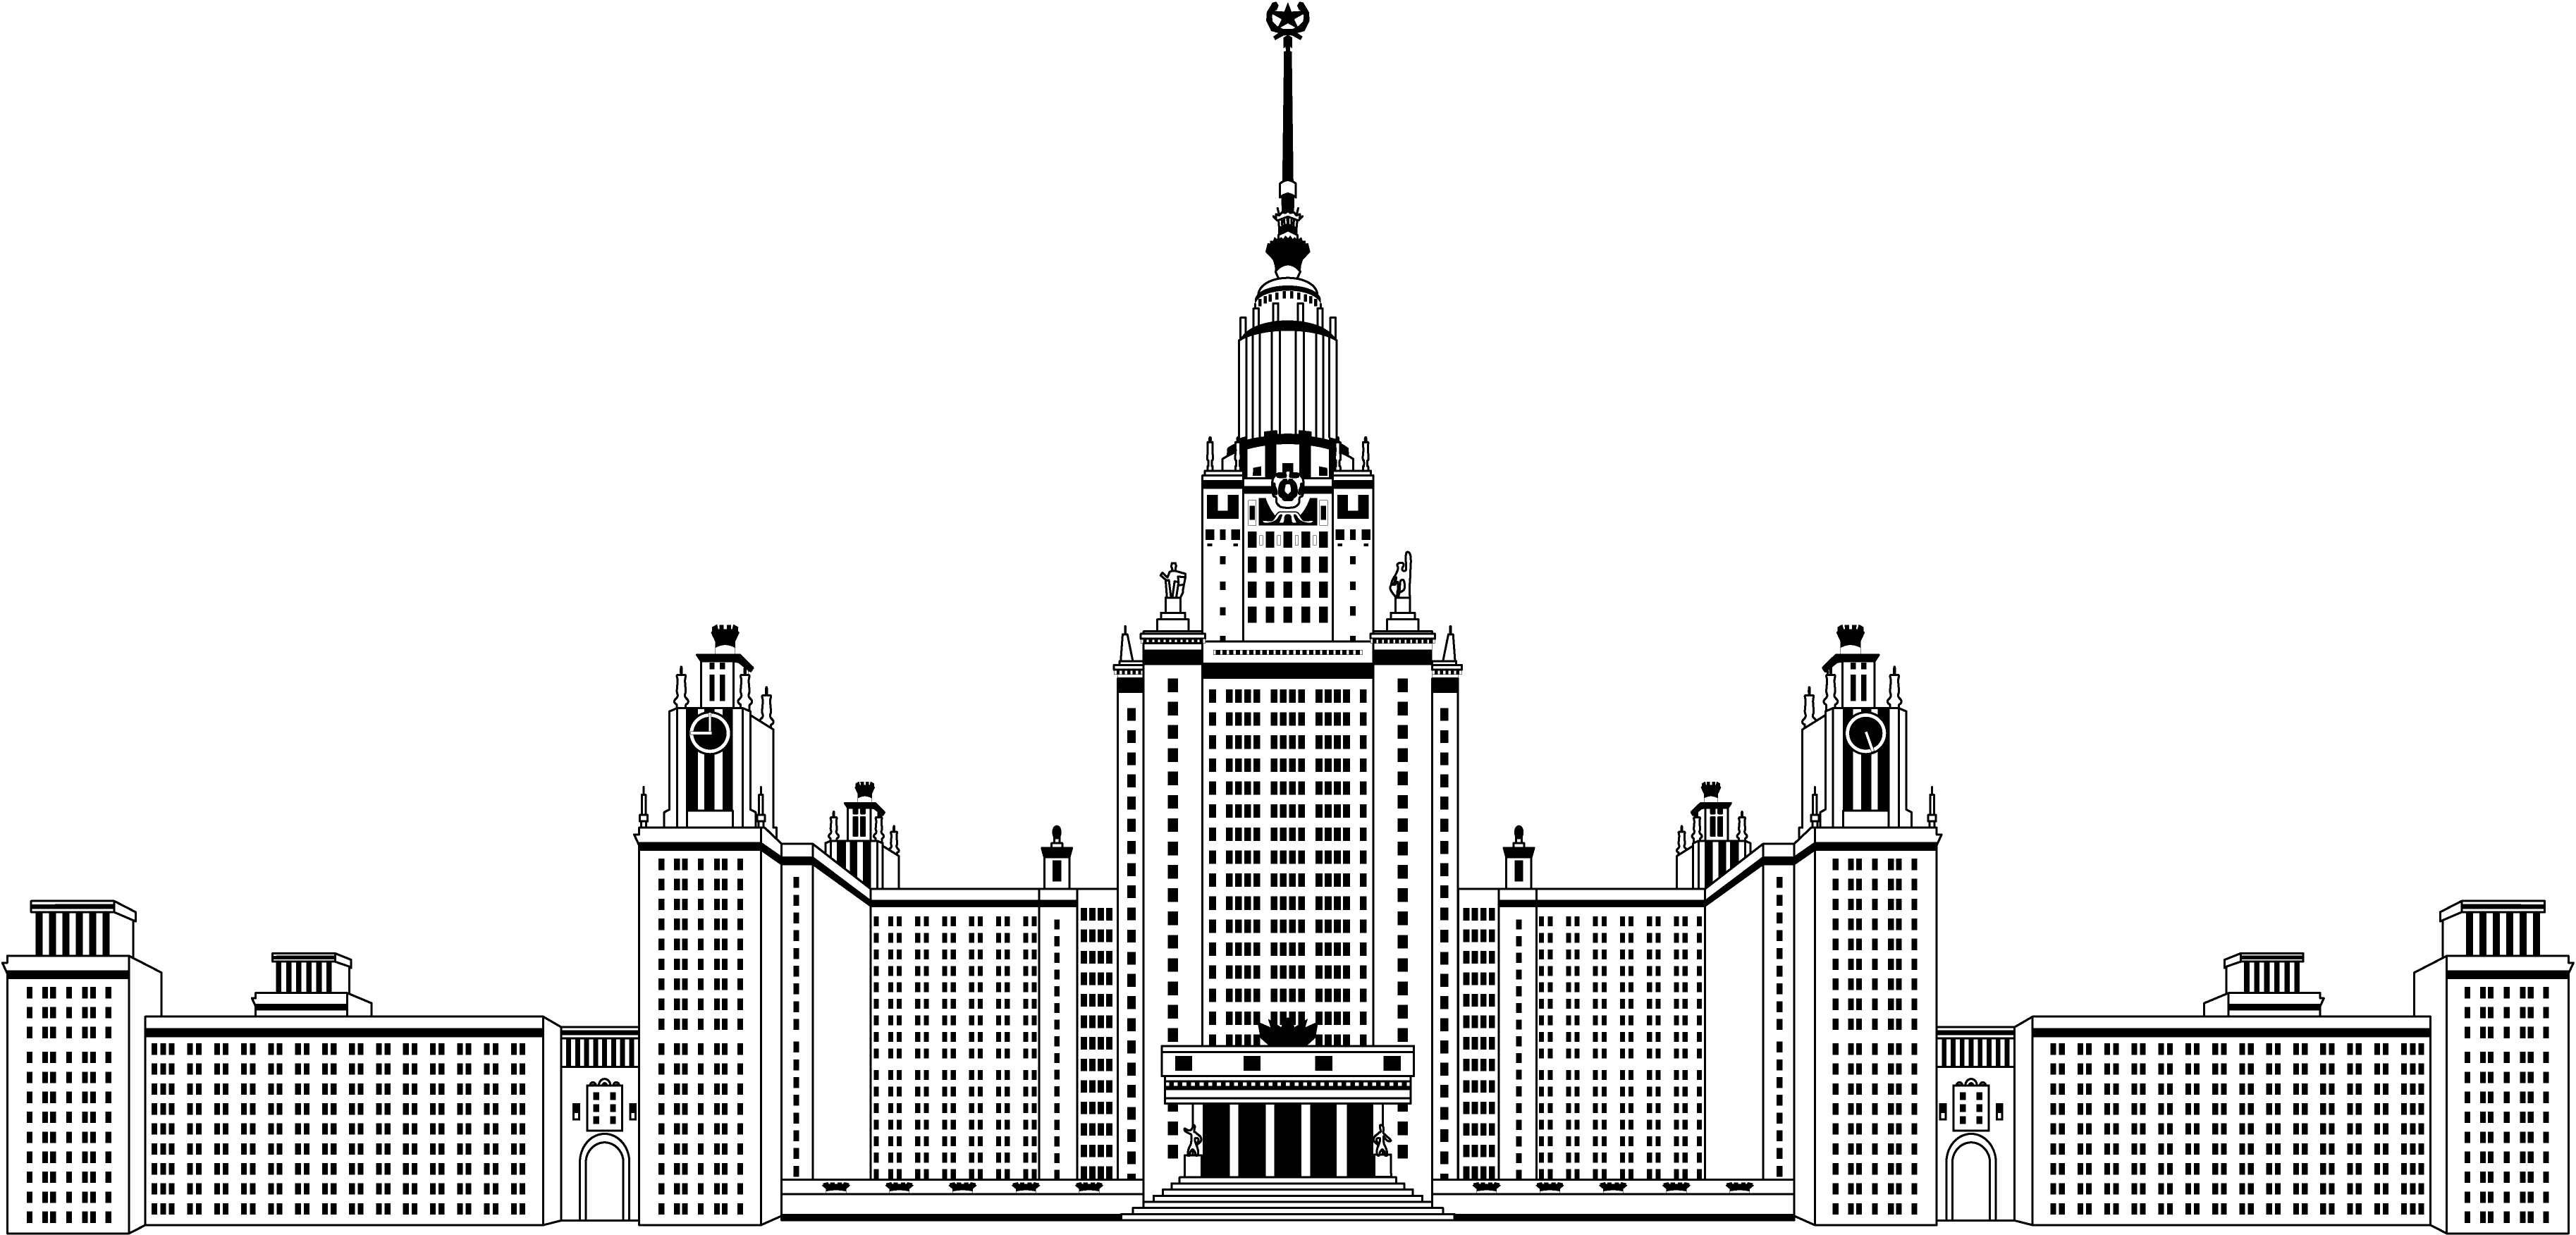
\includegraphics [width = 0.5 \textwidth] {msu.png} \\
    {\scshape Московский Государственный Университет} \\
    Факультет вычислительной математики и кибернетики\\

    \vspace {5cm}

    % {\LARGE Отчет}

    % \vspace {1cm}

    {\Huge \bfseries
    <<Отчет о выполнении задания на ПВС>> \\}
\end {center}

\vfill
\vfill

\begin {flushright}
    \large
    Гордеев Михаил \\
    студент группы 618/1 \\
    вариант 2 \\

    \vspace {5mm}
\end {flushright}

\vfill

\begin {center}
    Москва, 2016
\end {center}

\enlargethispage {4 \baselineskip}

\newpage

\section{Математическая постановка дифференциальной задачи} В прямоугольной
области $[0,1] \times [0,1]$ требуется найти дважды гладкую функцию $u =
u(x,y)$, удовлетворяющую дифференциальному уравнению $$ -\Delta{u} = 4(2 - 3x^2
- 3y^2), 0<x<1, 0<y<1 $$ и дополнительному условию $u(x,y) = (1-x^2)^2 +
(1-y^2)^2$ во всех граничных точках $(x, y)$ прямоугольника.  Оператор Лапласа
$\Delta$ определен равенством: $$ \Delta{u} = \frac{\partial^2u}{\partial{x^2}}
+ \frac{\partial^2u}{\partial{y^2}} $$ Решением данной задачи является функция
$u(x,y) = (1-x^2)^2 + (1-y^2)^2$.


\section{Описание гибридной реализации}
При распараллеливании программы использовалось двумерное разбиение области на
подобласти прямоугольной формы.  Каждой прямоугольной подобласти соответствует
один MPI процесс. Процессам необходимо взаимодействовать друг с другом, так
как для вычисления пятиточечного разностного оператора Лапласа необходимо знать
значения функции p в соседних точках, а для граничных точек соседями могут
являться точки другой подобласти. Внутри одной подобласти вычисления
распараллеливаются с помощью OpenMP .

\newpage
\section{Результаты}
\subsection{Таблицы}

\begin{table}[htb]
    \centering
    \caption{Результаты расчетов на ПВС IBM Blue Gene/P MPI}
    \begin{tabular}{|r|r|r|r|}
        \hline
        Число процессоров $N_p$ & Число точек сетки $N^3$ & Время решения T & \
            Ускорение S \\ \hline
        % T1 5.32                                                            
        $128$ & $ 1000 \times 1000 $ & 0.14 & 38 \\ 
        $256$ & $ 1000 \times 1000 $ & 0.1 & 53.2 \\ 
        $512$ & $ 1000 \times 1000 $ & 0.09 & 59.1 \\ \hline
        % T1 63.29
        $128$ & $ 2000 \times 2000 $ & 0.53 & 119.42 \\ 
        $256$ & $ 2000 \times 2000 $ & 0.29 & 218.24 \\ 
        $512$ & $ 2000 \times 2000 $ & 0.2 & 316.45 \\ \hline
    \end{tabular}
\end{table}
\begin{table}[htb]
    \centering
    \caption{Результаты расчетов на ПВС IBM Blue Gene/P MPI/OpenMP}
    \begin{tabular}{|r|r|r|r|}
        \hline
        Число процессоров $N_p$ & Число точек сетки $N^3$ & Время решения T & \
            Ускорение S \\ \hline

        % Inaccuracy 0.006
        % T1 12.6
        $128$ & $ 1000 \times 1000 $ & 0.09 & 140 \\ 
        $256$ & $ 1000 \times 1000 $ & 0.07 & 180 \\ 
        $512$ & $ 1000 \times 1000 $ & 0.07 & 180 \\ \hline

        % Inaccuracy 0.01
        % T1 = 26.24
        $128$ & $ 2000 \times 2000 $ & 0.25 & 104.96 \\ 
        $256$ & $ 2000 \times 2000 $ & 0.16 & 164 \\ 
        $512$ & $ 2000 \times 2000 $ & 0.12 & 218.67 \\ \hline
    \end{tabular}
\end{table}


\newpage
\subsection{Графики}
\begin{figure}[h]
    \centering
    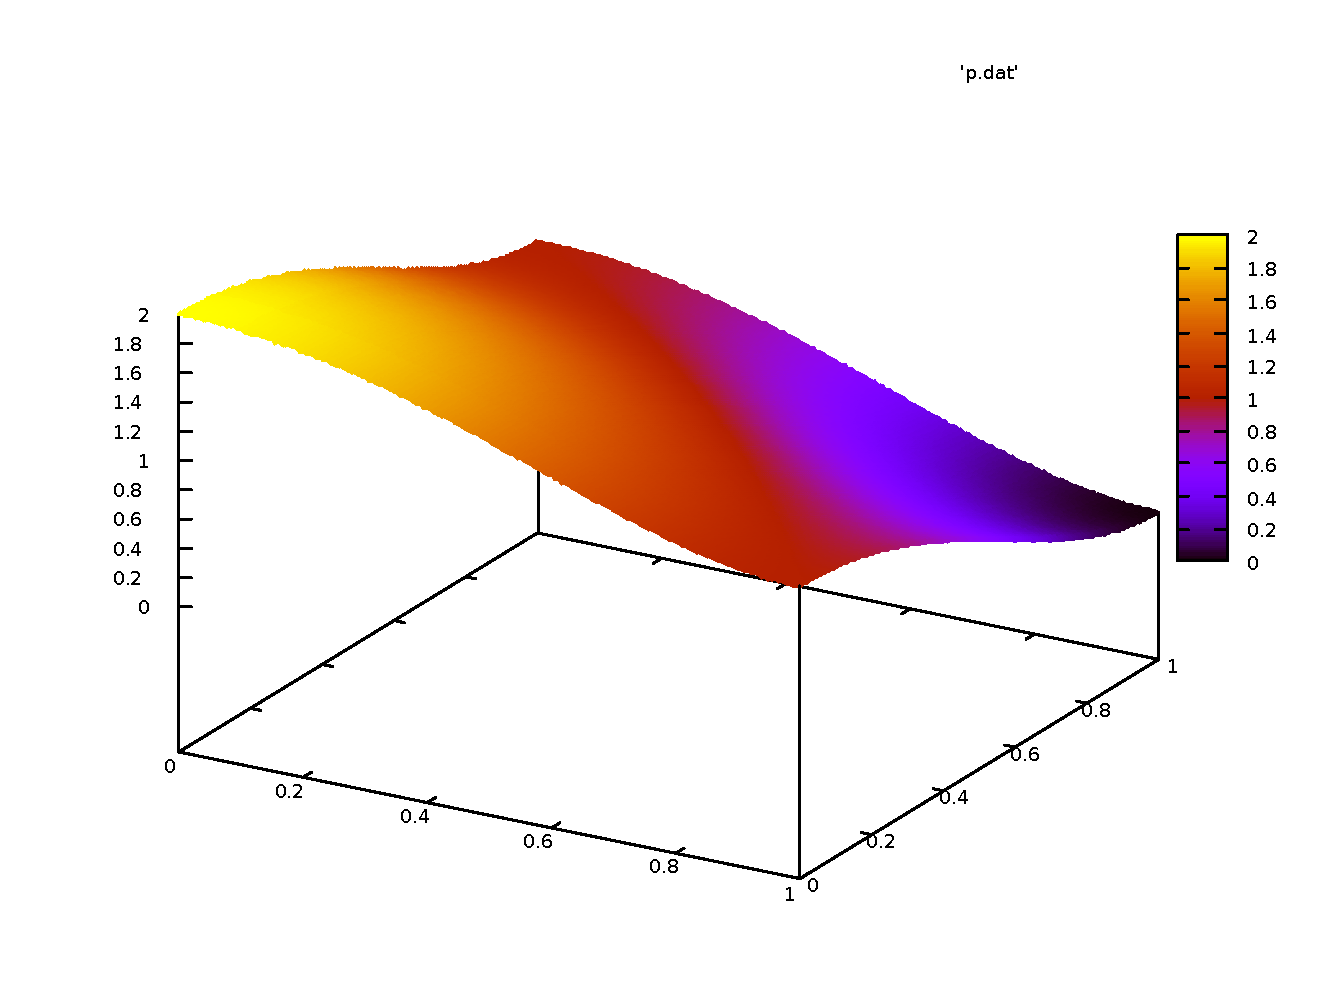
\includegraphics[height=185pt, width=185pt]{p.pdf}
    \caption{Приближенное решение, полученное программой}
\end{figure}
\begin{figure}[h]
    \centering
    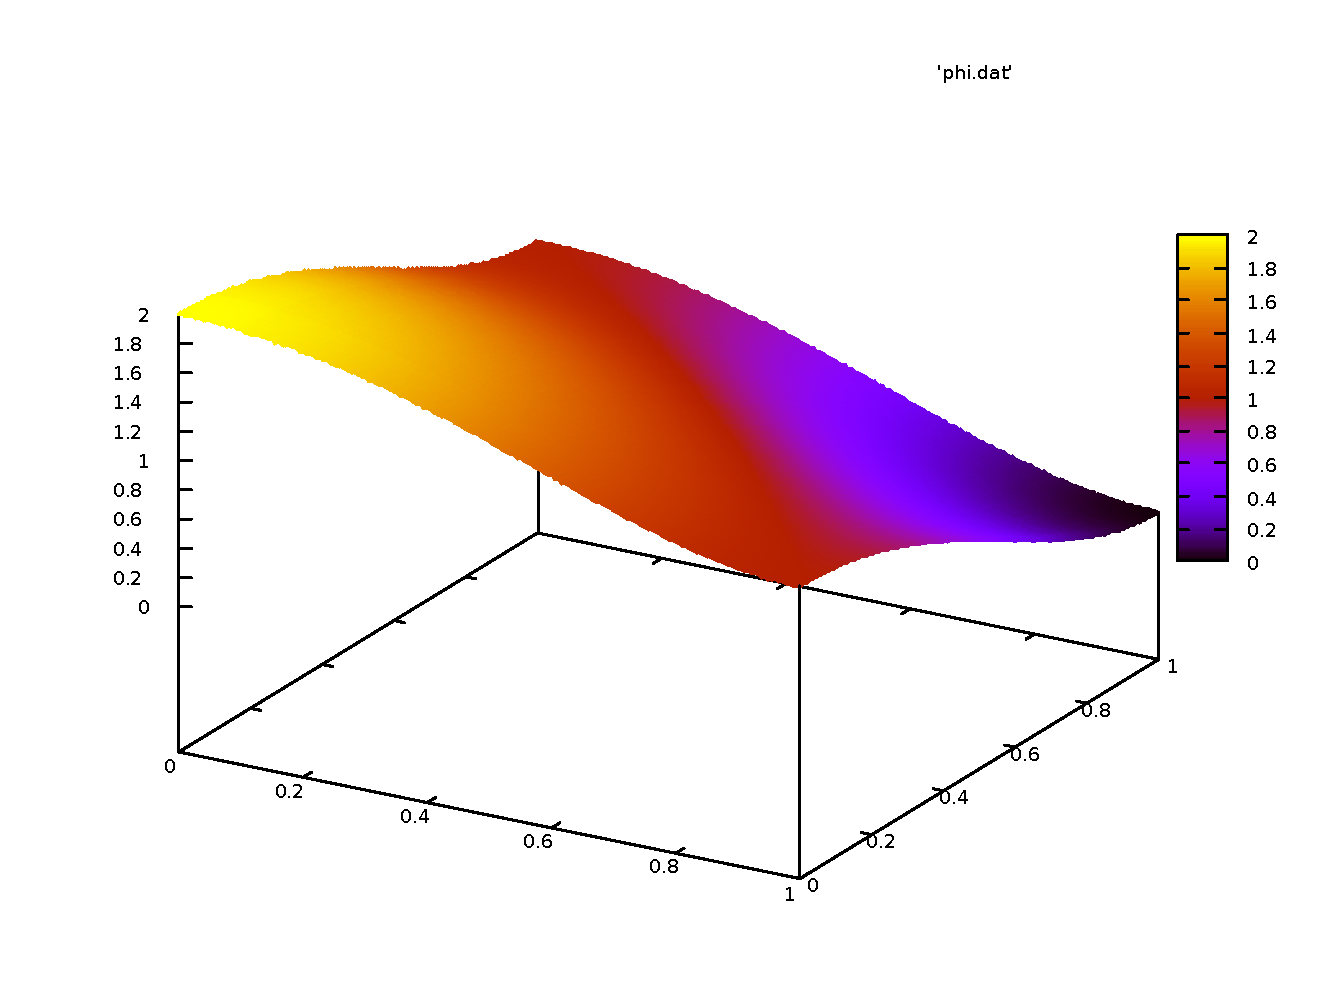
\includegraphics[height=185pt, width=185pt]{phi.pdf}
    \caption{Точное решение}
\end{figure}
\end {document}
